\chapter{Multiwibrator astabilny}

\section{Budowa układu}

\begin{itemize}
    \item Do budowy układu posłużono się schematem (\ref{fig:schemat_multiwibratora}) oraz dodatkowym kondensatorem, rezystorem oraz dwoma rezystorami znajdującymi się na płytce.
    \item Wartości użytych elementów:
        \begin{gather}
            \label{multiwibrator:C} C = \textbf{21.9nF} \\
            \label{multiwibrator:Rf} R_f = \textbf{0.99k\boldsymbol{\Omega}} \\
            \label{multiwibrator:R1} R_1 = \textbf{85.9\boldsymbol{\Omega}} \\
            \label{multiwibrator:R2} R_2 = \textbf{1k\boldsymbol{\Omega}}
        \end{gather}
    \item Zbudowany układ:
        \begin{figure}[H]
            \centering
            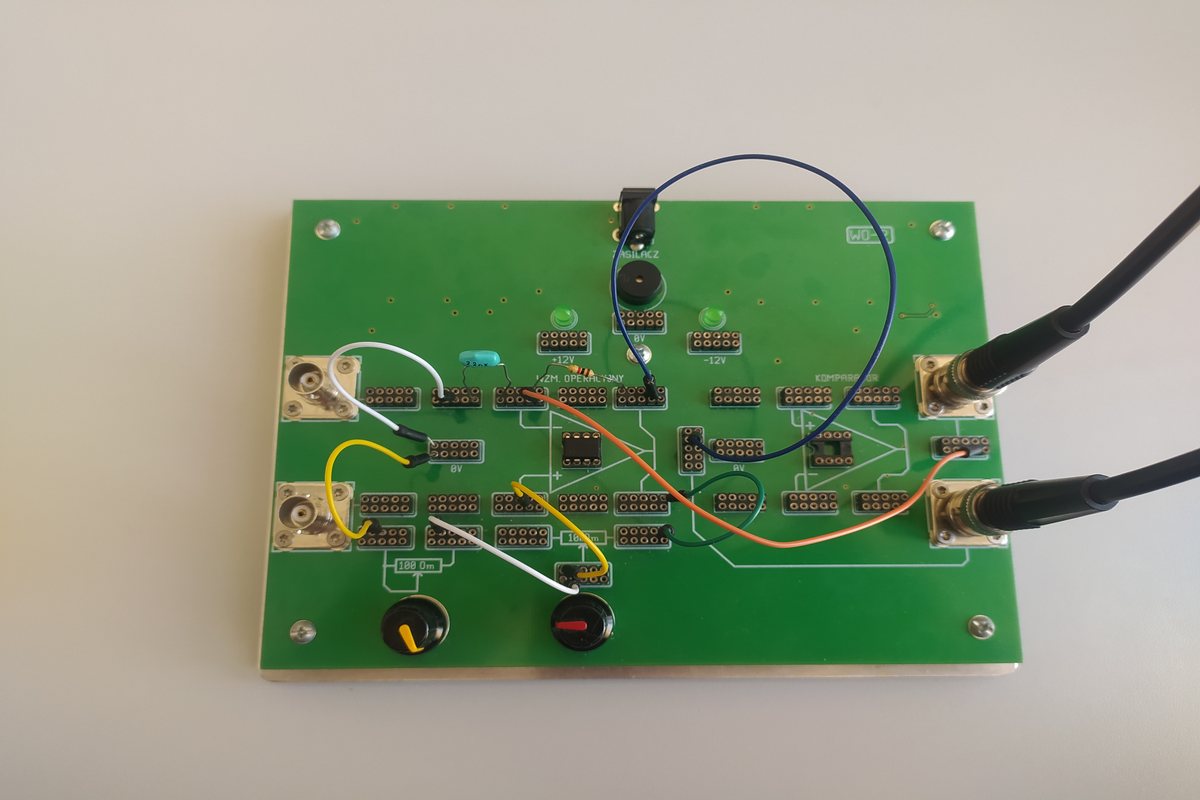
\includegraphics[scale=0.17]{img/phone/1651502036773_scaled.png}
            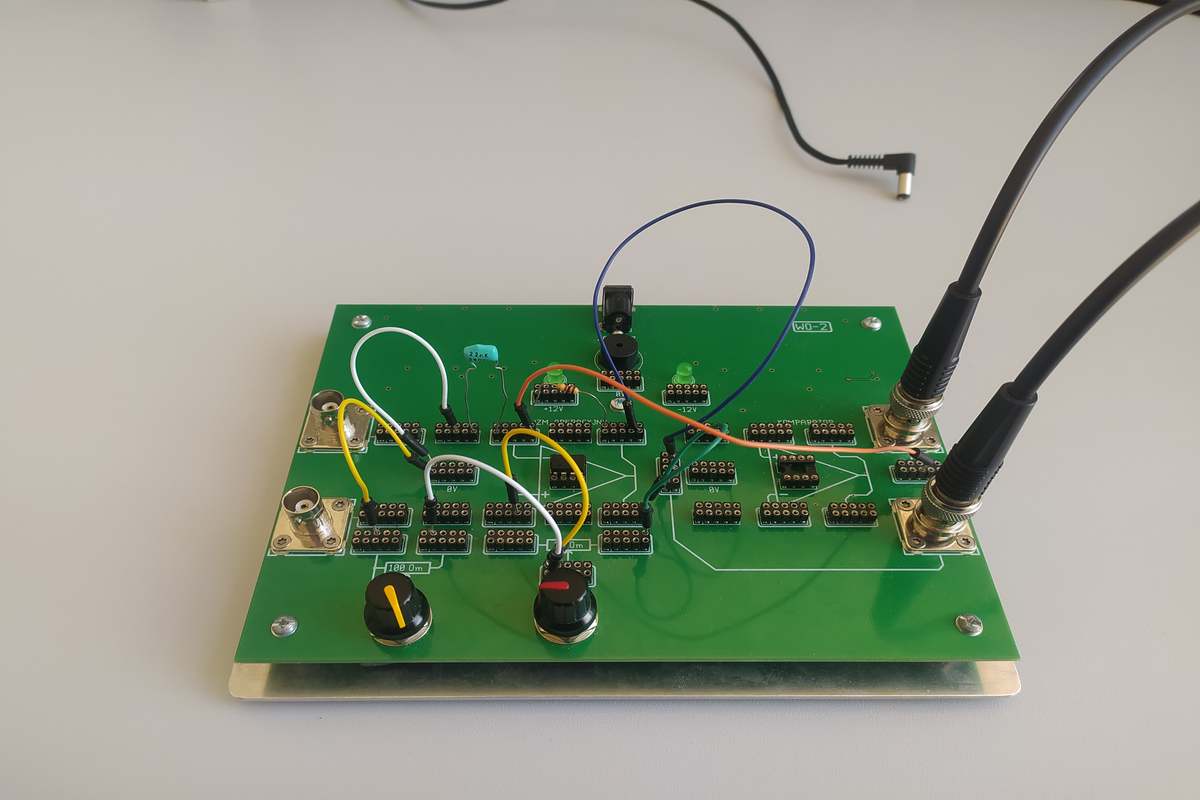
\includegraphics[scale=0.17]{img/phone/1651502036761_scaled.png}
            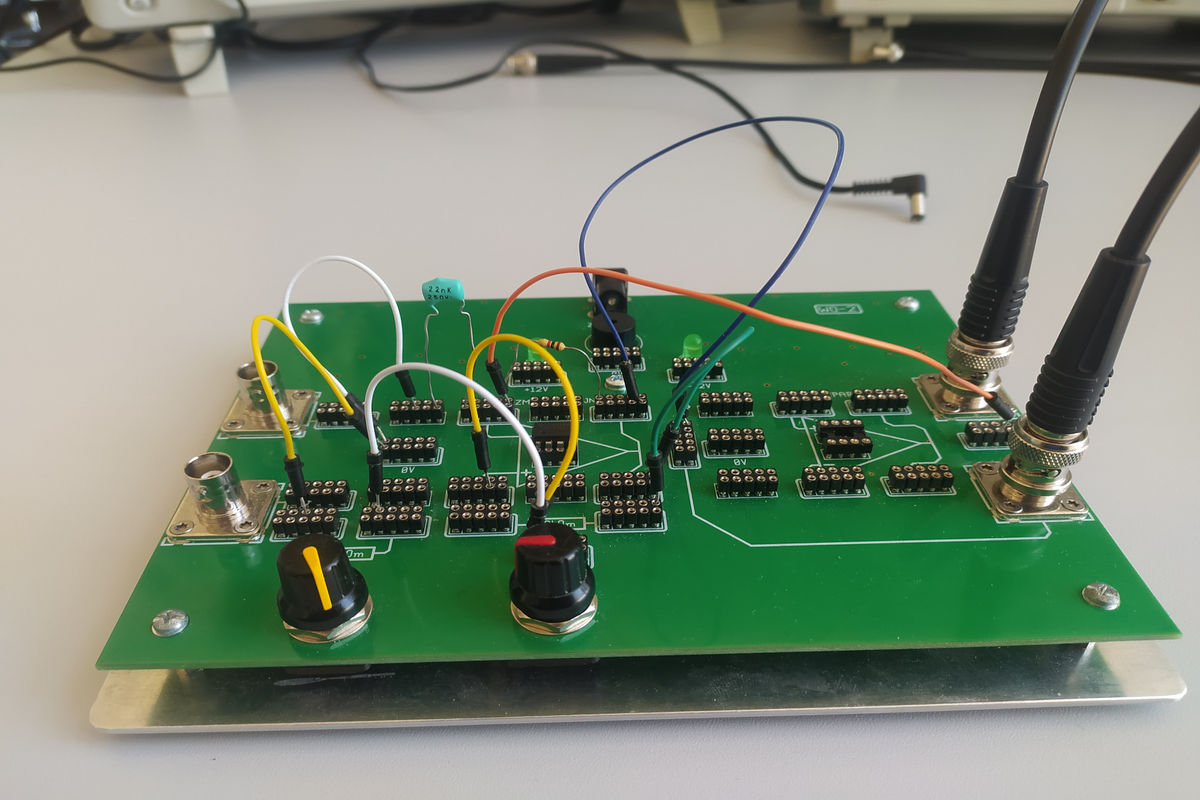
\includegraphics[scale=0.25]{img/phone/1651502036744_scaled.png}
            \caption{Zbudowany multiwibrator astabilny}
            \label{fig:multiwibrator_astabilny}
        \end{figure}
\end{itemize}

\pagebreak

\section{Przebieg impulsu}

\begin{itemize}
    \item Teoretyczny przebieg:
        \begin{figure}[H]
            \centering
            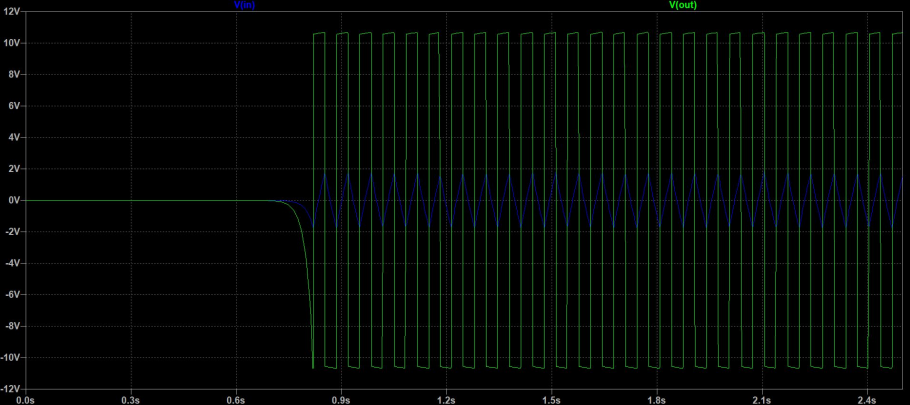
\includegraphics[width=\textwidth]{img/theoretical/multiwibrator_przebieg.png}
            \caption{Teoretyczny przebieg impulsu}
            \label{fig:multiwibrator_teor_przebieg}
        \end{figure}
    \item Doświadczalny przebieg (kanał 1 - sygnał w punkcie \textbf{1}, kanał 2 - wyjście multiwibratora \textbf{Wy} (\ref{fig:schemat_multiwibratora}):
        \begin{figure}[H]
            \centering
            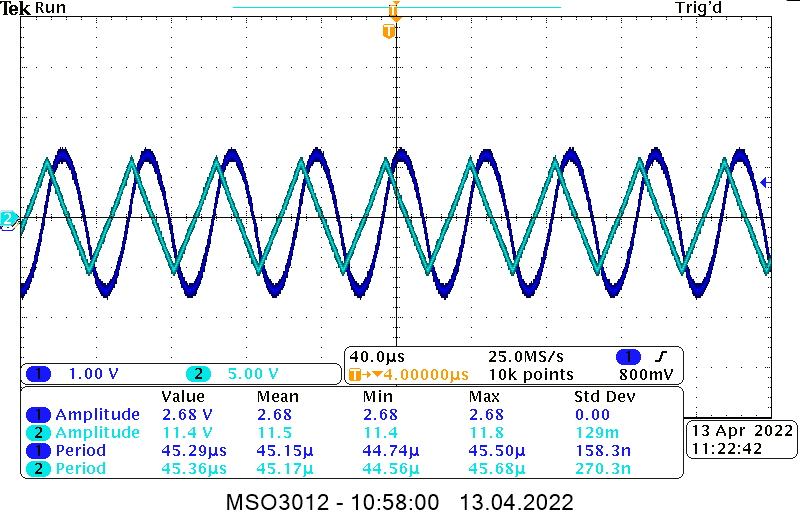
\includegraphics[width=\textwidth]{img/osciloscope/1_5_period_cropped.png}
            \caption{Doświadczalny przebieg impulsu}
            \label{fig:multiwibrator_dosw_przebieg}
        \end{figure}
    \item Doświadczalny przebieg impulsu zgadza się z teoretycznym.
\end{itemize}

\section{Pomiary}

\begin{itemize}
    \item Wyliczono wartość teoretyczną okresu drgań za pomocą wzorów (\ref{eq:multiwibrator_okres_drgań}, \ref{eq:multiwibrator_gamma}):
        \begin{equation}
            \gamma = \dfrac{R_2}{R_1+R_2} = \dfrac{1k\Omega}{85.9\Omega + 1k\Omega} = \textbf{0.92} \\
        \end{equation}
        \begin{equation}
            T_{teor} = 2 R_f C \ln({\dfrac{1+\gamma}{1-\gamma}}) = 2 \cdot 1k\Omega \cdot 21.9nF \cdot \ln({\dfrac{1.92}{0.08}}) = \textbf{140.28\boldsymbol{\mu}s}
        \end{equation}
    \item Wykonane pomiary:
        \begin{figure}[H]
            \centering
            \begin{subfigure}[h]{0.49\textwidth}
                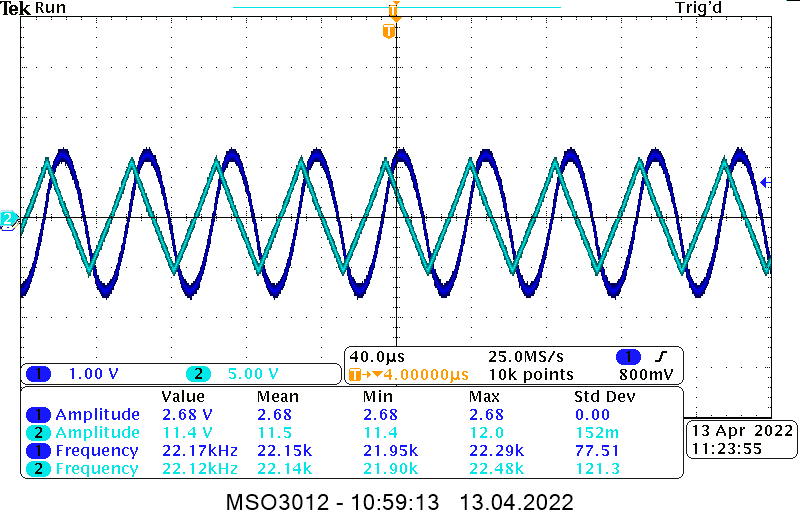
\includegraphics[width=\textwidth]{img/osciloscope/1_5_freq_cropped.png}
                \caption*{Pomiar częstotliwości}
            \end{subfigure}
            \begin{subfigure}[h]{0.49\textwidth}
                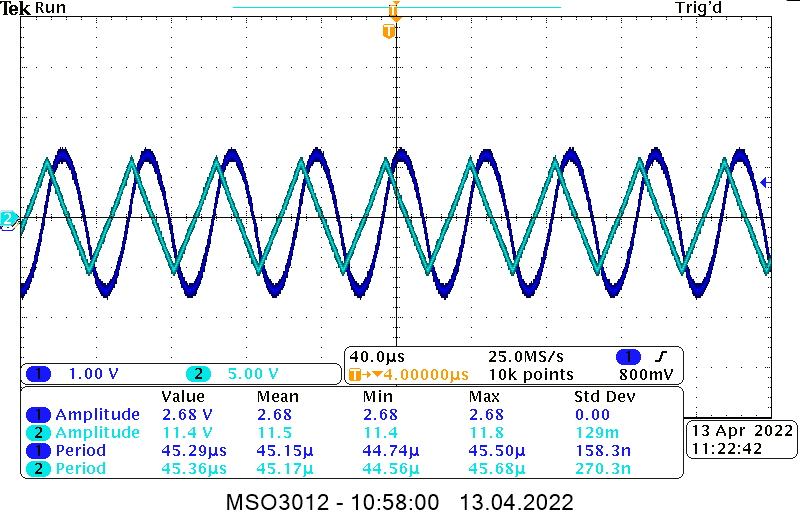
\includegraphics[width=\textwidth]{img/osciloscope/1_5_period_cropped.png}
                \caption*{Pomiar okresu}
            \end{subfigure}
            \label{multiwibrator:pomiar}
        \end{figure}
    \item Eksperymentalna wartość okresu wyniosła:
        \begin{gather}
            T_{eksp} = \textbf{45.29\boldsymbol{\mu}s}
        \end{gather}
    \item Różnica między wartością teoretyczną okresu a uzyskaną eksperymentalnie wyniosła:
        \begin{gather}
            \Delta_T = T_{teor} - T_{eksp} = \textbf{94.99\boldsymbol{\mu}s} \\
            \delta = \dfrac{\Delta_T}{T_{teor}} \cdot 100\% \approx 67.7\%
        \end{gather}
    \item Duża różnica między wartością teoretyczną a doświadczalną prawdopodobnie spowodowana jest błędem pomiaru któregoś z użytych elementów (\ref{multiwibrator:C}, \ref{multiwibrator:Rf}, \ref{multiwibrator:R1}, \ref{multiwibrator:R2}) oraz brakiem czasu na dokładniejsze pomiary spowodowanym końcem laboratoriów.
\end{itemize}